\chapter{Welcome}
\section{Abstract}
\xmlswing\ is a tool to create swing templates based on a
XML file. The developer provides a XML file and the software
will create a source code (not a compiled class) with all
the stuff necessary to have a graphic user interface in Swing.

The main difference with other tools proposed are:
\begin{itemize}
  \item Provides a JAVA source code.
  \item Integrates ``out-of-the-box'' features (look and
  		feel menu, etc.)
  \item Some helpful way to manage the AWT-Thread.
  \item Components organized on a HTML \verb|<table>| style (alignments,
  			grouping, etc.).
  \item Native SWING components extensions are possible.
\end{itemize}


\section{Using native interface}
Now, there are many providers giving you good solutions to create
your own GUI. The idea behind the \xmlswing{} is to give a way
for writing simple graphic interfaces very fast. Not only the
display itself but also programming a SWING application.


The program will help to create plain JAVA source code you have to
extend with your own class. You should NEVER use directly the code generated
by the program. Creating an GUI using the swing library is a natural
choice for creating basic things. If you want beautiful and more than
modern graphical interfaces, use JavaFX instead (but be careful, it is not 
part of the OpenJDK project and subject to licences). We just provide a
basic software with an open source code.

You simply have to provide all the things to put together in your GUI.
Only give names to components you want to control
(as a \verb|JTextField|). Menus can be generated quickly (and XML is
the best way to describe them): for each menu, you simply give the method
for processing the code behind.
 

About the licence: you can use this software for any purpose. The generated
classes can be distributed in binary mode or with the source code included. When
your development provides the \verb|.java| code source, it must be also
provide the \verb|.xml| file used to generate it (if possible in the
same directory or in the resource directory if you use Maven). This is typically non sense to distribute the source code
generated by this software but without the original XML file.

Note some of the functionalities described in this document
may be not yet implemented. Send me a request directly if needed.

\section{How it works}
You write an XML file containing the GUI interface you want. Normally, only
the graphical part is expressed in this file. Once the XML file is ready, you
run the software and it will generate a \JAVA\ code source in the
right directory (you can specify the directory in arguments). The class created
includes a \jmethod{main} method to test the graphical interface but you
have to create your own class based on the generated one to add the logic.
 

The generated class includes:
\begin{itemize}
  \item A \jmethod{main} method for test purposes.
  \item A \jmethod{initComponents} method for initializing the graphical objects.
\end{itemize}


That's quite simple. Do not try to understand the generated code, I can
just say: ``It works'' but the swing implementation is a confusion addition
of multiple things including menus, components, layouts and some other
stuff.

\section{My first application}

\subsection{Create the frame}
Usually, all the GUI applications run into a \jclass{JFrame} object.
It is the base of our XML file. Write the code of the figure \ref{fig:first-jframe}.
It will create a very simple frame but with all the stuff needed.

\begin{figure}[htb]
\begin{lstlisting}[language=XML]
<?xml version="1.0" encoding="ISO-8859-1"?>

<JFrame 
  title="First frame" 
  name="com.oxande.xmlswing.example.AbstractSampleFrame"
  coolsize="300,150"
  icon="./forward16.gif">
</JFrame>

\end{lstlisting}
\caption{The minimal application}\label{fig:first-jframe}
\end{figure}

Of course, in respect of object abstracting, you should not use
the frame like this. Please create the following code to support
the frame.

\begin{figure}[htb]
\begin{lstlisting}[language=java]

package com.oxande.xmlswing.example;

public class SampleFrame extends AbstractSampleFrame {
}

\end{lstlisting}
\caption{The minimal implementation}\label{fig:first-java}
\end{figure}

If you use the same package than the frame object, it is
quite easy to support the graphical part. Now, you have to configure 
the \xmlswing\ program to generate the code. Then you have to
run it as follow (we consider you are in the root of your Maven 
workspace, where is stored the \verb|pom.xml| file):


\small
\begin{verbatim}
java -cp xml4swing.jar
     -d . 
     ./src/main/resources/com/oxande/xmlswing/example/tutorial.xml
\end{verbatim}
\normalsize

Then to run the sample created, please run your code as follow
(do not forget to add the root of your classes to your class path):
\small
\begin{verbatim}
java -cp ./target/classes
     com.oxande.xmlswing.example.example.SampleFrame
\end{verbatim}
\normalsize

And, the first application is created and display something
similar to what you have in figure \ref{fig:tuto-1}. It is the
first but quickly (I suppose) created application.


\begin{figure}[htb]
\begin{center}
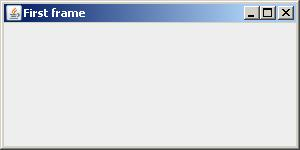
\includegraphics[width=0.5\linewidth]{tuto-1.jpg}
\end{center}
\caption{My first Application\label{fig:tuto-1}}
\end{figure}

Then, of course, it is very simple. Notice we didn't provide
the \verb|main| method for the application as we use the inherited one.
It is a good idea to create its own (figure \ref{fig:main}). You should
first instantiate the class. Then you initialize the components. In the last part, you set the frame to the visible mode.

\begin{figure}[htb]
\begin{lstlisting}[language=java]
public class SampleFrame extends AbstractSampleFrame {
   public static void main(String[] args)
   {
      SampleFrame appl = new SampleFrame();
      appl.initComponents();
      appl.setVisible(true);
   }
}
\end{lstlisting}
\caption{The main}\label{fig:main}
\end{figure}

Be careful, if you do this, when you close the window, the application
remains active. One way is to set the default close mode to
\verb|EXIT_ON_CLOSE|. But you have not to add new code: simply
add a tag to the XML file for the \emph{onClose} event. This event
is trigerred when the window is closed (i.e. the frame). See figure
\ref{fig:onclose} for the code added. It is quite simple, no? Now, your
application closes.

\begin{figure}[htb]
\begin{lstlisting}[language=XML]
<JFrame ...>
  <onClose>
     System.exit(0);
  </onClose>
</JFrame>
\end{lstlisting}
\caption{The minimal application}\label{fig:onclose}
\end{figure}

Another way to do is to use an attribute rather than the code
directly in the XML file. In this case, simply use the attribute
\verb|onClose="exit"| to give a method rather than the code.
You just have to implement this functionality by providing a
method as shown in figure \ref{fig:exitMethod}. Do not forget to
provide the method, if not the program will provide a default one
which throws an \verb|UnsupportedOperationException|.

\begin{figure}[htb]
\begin{lstlisting}[language=java]
public void exit(){
  System.exit(0);
}
\end{lstlisting}
\caption{The exit method}\label{fig:exitMethod}
\end{figure}

Now, you want to add a menu. Very simple, provide one as
cascaded menus in the XML file. Of course, we provide not
implemented ones. Each time, we provide a menu, the system
provide a default implementation showing a message saying it
is not implemented.

\begin{figure}[htb]
\begin{lstlisting}[language=XML]
<JFrame ...>
	<menubar>
    <menu>
      _File
			<item action="openFile">_Open File</item>
			<item>Close Fil_e</item>
			<separator />
			<item perform="exit">Exit</item>
		</menu>
		<menu>
			Help
			<lookandfeel />
    </menu>
  </menubar>
</JFrame>
\end{lstlisting}
\caption{The menu bar}\label{fig:menubar}
\end{figure}

The menu bar is simple. If you add \verb|action|s, you will
have something behing the menu. Note the ``\verb|_|'' (underscore)
sign to specify what letter will be underlined when the user
clicks on Alt button (for keyboard access). You should pay
attention to \verb|<separator/>| to simply create separators
and \verb|<lookandfeel/>| to have a complete menu to change
the look and feel of the application (evrything imported).

Note the \verb|action| attribute which points to the same \jmethod{exit}
method when the user close the window or select the \textit{Exit}
menu item.

\begin{figure}[htb]
\begin{center}
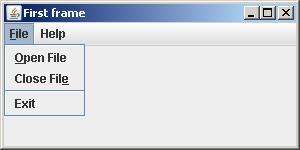
\includegraphics[width=0.5\linewidth]{tuto-2.jpg}
\end{center}
\caption{My first menu\label{fig:tuto-2}}
\end{figure}


\subsection{Add a status bar}

But, it is not the only the remarquable part. Now simply add the tag
\verb|<statusbar| \verb|id="statusBar"| \verb|property="statusMessage"| \verb|/>| and you have a status bar. Simply use the bean property
to set the message. You can write in your code \verb|setStatusMessage(msg)|
to change the status message. More than this, the change of the text is
made in the AWT-Thread because the text is changed by calling the
correct JAVA code to avoid an issue if you try to change the text
outside the AWT thread.

That's a king of magic. And the same is valid for the text objects
(\jclass{JTextArea}, \jclass{JTextField}, etc.) where the fact to set
the property permit to set it easily. But, please, don't look at the code
behind, it is a mess\ldots


\subsection{Add a toolbar}
As simple as for status bar, use the tag \verb|<toolbar>|
to add a toolbar (see section \ref{sec:JToolBar} for details).

\section{\label{sec:args}Arguments}
As for other JAVA programs, you must call the software using
the jar file (\verb|xml4swing.jar|) provided as follow:
\verb|java -cp xml4swing.jar| or add the jar file in the classpath
variable.

The complete command line becomes:
\verb|java -cp| \verb|xml4swing.jar| \verb|<arguments>| \verb|<templates>| where \verb|<arguments>| are the arguments shown below
and \verb|<templates>| the XML files which describe the different classes
to create. Using \verb|-| (the minus sign) as \verb|<templates>| will
use the standard input as XML file.


Please find below the arguments you can pass to \xmlswing:
\begin{itemize}
  \item \verb|-d <dir>|: the directory for sources. It is the base
  		of all your classes (basically \verb|${project_loc}/src/main/java|
  		if you use Maven.
  \item \verb|-V|: include the version. If set, a Javadoc tag
      \verb|@version| followed by the current date and time is added 
      in the source code of the class (do not use if you already have 
      a version control program as CVS or Subversion).
\end{itemize}

